\chapter{Documentation}

\section{Data Representation}
\begin{description}
\item [{\tt btRigidBody}]
\item [{\tt irr::scene::ISceneNode}]
\item [{\tt irr::scene::IMesh}] -buffers
\item [{\tt CGAL::Nef\_polyhedron\_3}]
\item [{\tt gg::MObject}]
\end{description}


\section{Input data}
\label{sec:data}
.obj/.3ds
describe format in world file

\section{Modules}
In this section, we describe the functionality of each program module. Third party software will not be described here. It can be found in \cref{chapt:technology}. Interactions between modules are described in \cref{fig:modules}. \emph{Irrlicht Engine} is not present in the diagram because we do not logically depend on using this engine. Every module is implemented in a file with the matching name as a class with the same name prefixed with letter M (Object Creator can be found in file ObjectCreator.cpp and is implemented as class {\tt gg::MObjectCreator}). Every component of this application is located in namespace {\tt gg};

\begin{figure}[ht!]
        \centering
        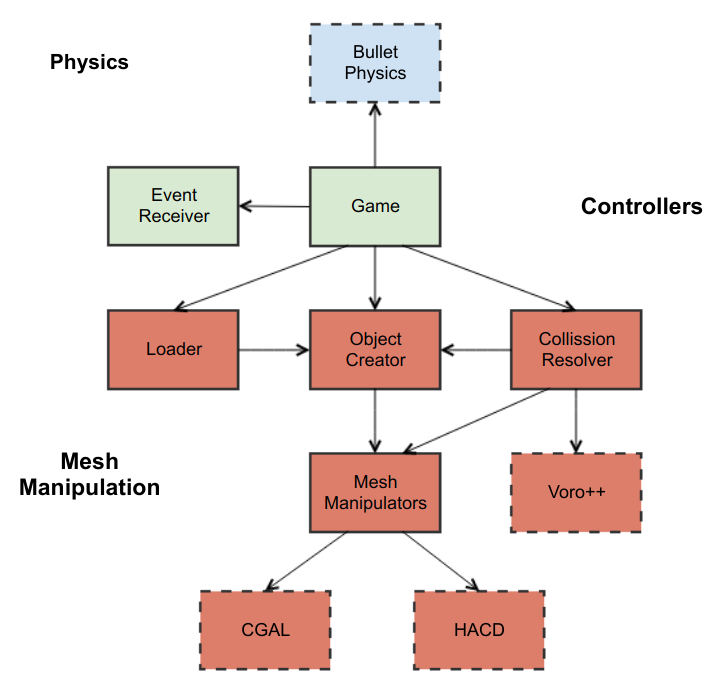
\includegraphics[width=\textwidth]{img/objectmodel}
        \caption{Software architecture shown on diagram of relationships of program modules. Third party software is highlighted in dashed rectangles.}
        \label{fig:modules}
\end{figure}

\begin{description}
\item[Game]
The {\tt gg::MGame} class is the core of application. 

\item[Event Receiver]
This class is an implementation of {\tt irr::IEventReceiver} from Irrlicht engine and it is used to read the user input.

\item[Loader]
The Loader is a class only used for initializing the application. It parses the data describing the game environment from the given file, constructs the objects with the help of {\tt gg::MObjectCreator} and returns the set of constructed objects.

\item[Object Creator]
We use this class as a Builder pattern in order to initialize the data contained inside {\tt gg::MObject} ({\tt CGAL::Nef\_polyhedron\_3, btRigidBody, irr::scene::ISceneNode}).

There are three member functions allowing us to create {\tt gg::MObject}s  with different behaviour from the same set of input parameters (see \cref{sec:data}). We can achieve destructible object, indestructible objects with box collision shape and rectangular indestructible object without input mesh. Those functions are exclusively used at initialization as they generate a new set of member variables and their parameters come in a text form.

Two more kinds of objects can be created. A projectile that is shot from the given position with the given impulse. And a destructible object with temporary collision shape (sphere shaped). Because this object is constructed whilst game is being played and construction of {\tt CGAL::Nef\_polyhedron\_3} can take a longer time, it requires to have the {\tt CGAL::Nef\_polyhedron\_3} given in parameter.

\item[Collision Resolver]
\todo{All the magic happens here!}

\item[Mesh Manipulators]
Mesh Manipulators provides set of public static functions. Because different libraries are used for physics simulation, rendering and geometric manipulation, those functions provide means for converting data between different formats.
\end{description}



\section{Installation guide}

\section{User interface}
The user interface allows only for the use of the keyboard as follows:
\begin{itemize}
\item W/S: pitch down/up
\item A/D: roll counter-clockwise/clockwise 
\item Q/E: yaw left/right
\item Z/X: speed up/slow down
\item Space Bar: shoot or unpause
\item P: pause the game
\item ESC: quit the game
\end{itemize}
Keys can be pressed simultaneously and also held down instead of multiple presses.

